
\documentclass{aq-notes}
% \usepackage{amsthm}
\usepackage{formal}
\usepackage{graphicx}
\usepackage{amssymb}
\usepackage{tikz}
\usepackage{tabularx}
% \theoremstyle{plain}% default
% \newtheorem{theorem}{Theorem}[section]
% \newtheorem{lemma}[theorem]{Lemma}
% \newtheorem{proposition}[theorem]{Proposition}
% \newtheorem*{corollary}{Corollary}


% \theoremstyle{definition}
% \newtheorem{definition}{Definition}[section]
% \newtheorem{example}{Example}[section]
% \newtheorem{xca}[example]{Exercise}

% \theoremstyle{remark}
% \newtheorem*{rem}{Remark}
% \newtheorem*{note}{Note}
% \newtheorem{case}{Case}
\title{\bf Language Theory}
\course{CSC240}
\author{Kunlong Wu}
\begin{document}
\section{Language}

    \begin{definition}[Language]
            Let $\Sigma$ denote a finite alphabet (a finite set of letters)\\
            A {\bf Language} over $\Sigma$ is a subset of $\Sigma^*$ i.e.,  a set of strings with letters in $\Sigma$.
    \end{definition}
    \begin{definition}[Concatenation Operator $``\circ "$]
        Suppose $L$ and $L'$ are Languages, then
        \[L\circ L' = LL' = \{x\cdot y | x\in L \mbox{ and } y\in L'\}\]
    \end{definition}
    \begin{example}
        Suppose $L= \{a,bb\}$ and $L'=\{\lambda, c\}$\\
        Then $LL' =  \{a,bb,ac,bbc\}$ and $L'L = \{a,bb,ca,cbb\}$
    \end{example}
    \begin{definition}[\/$\lambda$\/]
        For any string $x \in \Sigma^*$, we have $x\cdot \lambda = \lambda \cdot x  = x$
    \end{definition}

    \begin{remark}
        $L^0 = \{\lambda\} \neq \lambda$
    \end{remark}

    \begin{definition}[ $L^i, L^*, L^+$ ]
        \begin{align*}
            L^1 &:= L\\
            L^{i+1} &:= L^i \cdot  L = L\cdot  L^i\\
            L^* &:= \bigcup_{i = 0}^\infty L^i\\
            L^+ &:= \bigcup_{i = 1}^\infty L^i
        \end{align*}
    \end{definition}
    \begin{remark}
        $L^* =L^+$ iff $\lambda\in L$
    \end{remark}
    \begin{theorem}[association]
        \[\forall x,y,z\in \Sigma^*. (xy)z = x(yz) = xyz\]
    \end{theorem}
    \begin{definition}[Prefix]
        $x$ is a {\bf prefix} of $y$ if there exists a string $x'$ such that $y = xx'$
    \end{definition}

    \begin{example}
        $\lambda$ and $y$ are prefixes of $y$
    \end{example}

    \begin{definition}[Suffix]
        $x$ is a {\bf suffix} of $y$ if there exist a string such that $y = x'x$
    \end{definition}

    \begin{definition}[Substring]
        $x$ is a {\bf substring} of $y$ if there exists strings $x'$ and $x''$ such that $x' xx'' = y$
    \end{definition}

    \begin{example}
        Let $y = aabaa$ and $x=aa$\\
        then x is prefix and suffix of y but $x \neq y$
    \end{example}


    \begin{definition}[Other operators on Language]
        If L and L' are languages over $\Sigma$ so are
        \[L\cup L', L\cap L', L-L', \overline{L} = \Sigma^* - L\] 
    \end{definition}


\newpage

\section{Regular Expressions}

    \begin{definition}[Regular Expression]
        Let $\Sigma$ be a finite alphabet (not include $+, *,\cdot, \lambda, \phi$)\\
        Let $R$ be the inductively defined set of strings(R is the set of {\bf regular Expressions} over $\Sigma$):\vspace{1ex}\\
        Base Case: $\emptyset, \lambda \in R,\ \Sigma \subseteq R$\\
        Constructor Cases: if $r,r'\in R$, then $(r+r')\in R, (r\cdot r')\in R, r^*\in R$
    \end{definition}

    \begin{definition}[Languages derived by $R$]
        The language derived by a regular expression is $\mathcal{L}(r)$ where 
        \[\mathcal{L}:R\to \{L|L\subseteq \Sigma^*\}\] which is defined inductively\\
        Base cases:
        \begin{align*}
            \mathcal{L}(\lambda) &:= \{\lambda\}\\
            \mathcal{L}(\emptyset) &:= \emptyset\\
            \mathcal{L}(a) &:= \{a\} \mbox{ for all } a \in \Sigma\\
        \end{align*}
        Constructor Cases:
        \begin{align*}
            \mathcal{L}((r+r')) &:= \mathcal{L}(r) \cup \mathcal{L}(r')\\
            \mathcal{L}((r\cdot r')) &:= \mathcal{L}(r)\cdot \mathcal{L}(r')\\
            \mathcal{L}(r^*) &:= \mathcal{L}(r)^*
        \end{align*}
        
    \end{definition}
    \begin{example}
        $((r_1\cdot r_2)\cdot r_3) = (r_1\cdot r_2\cdot r_3)$
        can remove ``( '' and ``)'' when no ambiguty
    \end{example}

    \begin{definition}[Regular Lang]
        A Language L is {\bf regular} if and only if $L=\mathcal{L}(r)$ for some regular expressions r.
    \end{definition}

    \begin{definition}[Equivalent of regular expression]
        Two regular expression r and $r'$ are {\bf equivalent} $r \equiv r'$ if and only if 
        \[\mathcal{L}(r) = \mathcal{L}(r')\]
    \end{definition}

    \begin{example}
        Let $L_0 = $ ``string over $\{a,b,c\}$ that start with $ab$'', then the regular expression of $L_0$ is
        \[a\cdot b\cdot (a+b+c)^*\]
        i.e., $\mathcal{L}(a\cdot b\cdot (a+b+c)^*) = L_0$
    \end{example}


    \begin{example}\label{L1}
        Let $L_1$ = ``strings over $\{0,1\}^*$ containing an even number of 1's'', then
        \[L_1= \mathcal{L}((0^*10^*1)^*0^*)\]
    \end{example}
    \begin{example}
        Let $L_2$ = ``first and last symbols are different $\subseteq \{0,1\}^*$'', then
        \[((0(0+1)^*1)+(1(0+1)^*0))\] 
    \end{example}
    \begin{theorem}
        Example \ref{L1} is true.\\
        i.e., Denote $L_1$ as ``strings over $\{0,1\}^*$ containing an even number of 1's'', then
        \[L_1= \mathcal{L}((0^*10^*1)^*0^*) = \mathcal{L}(r_1)\]
        \begin{proof}
            \begin{formal}
                \ul
            Let $x\in L_1$ be arbitrary \ul
                    \n  if $s\in \{0\}^*$ then \ul
                        \n  $s\in \mathcal{L}((0^*10^*1)^*0^*))$. \ul\p
                    Therefore\ul
                    If $x\in \mathcal{L}(0^*)$ \ul
                        \n then $x\in \mathcal{L}((0^*10^*1)^*0^*)$ \ul
                    \p  otherwise $x$ has at least two 1 \ul
                    \n  let $x_1$ be the shortest prefix of $x$ containing two 1  \ul
                        $x = x_1x'$ \ul
                        Let $x_1 = u1v1 $ where $u,v\in \{0\}^* \in \mathcal{L}(r_1)$\ul
    \ul
            Prove from induction on the \# of 1's in $x$ \ul 
            Let $P(n) = \forall x \in \{0,1\}^*. $(if $x$ contains exactly $2n$ ones then $x \in \mathcal{L}(r_1)$) \ul
            Suppose P(n) \ul
                \n Let $x\in L_1$ be an arbitrary string such that has $2n+2$ ones \ul\p
            By induction hypothesis,  \ul
                \n $x' \in \mathcal{L}(r_1) $, since $x_1$ has 2n ones. \ul
                so $x = x_1x'\in \mathcal{L}(0^*10^*1)\mathcal{L}((0^*10^*1)^*0^*)\subseteq \mathcal{L}((0^*10^*1)^*0^*)$ \ul\p
            Hence P(n+1) \ul
            By induction $\forall n \in \mathbb{N}. P(n)$\ul
    \p\p$L_1 \subseteq \mathcal{L}(r_1)$\ul
    \ul
            Suppose $x \in \mathcal{L}(r_1)$ \ul
            \n so $\exists k \in \mathbb{N}.x = (x_1...x_k)x'$ \ul
            where $x_i\in \mathcal{L}(0^*10^*1)$ for $1 \leq i \leq k$ and $x' \in \mathcal{L}(0^*)$ \ul
            Note that \# 1's in $x_i$ is exactly 2 \ul
            Number of 1's in $x'$ is 0 \ul
            Hence $x$ has even number of 1's  \ul
            i.e.,$ x\in L_1$ \ul
    \p $\mathcal{L}(r_1)\subseteq L_1$
            \end{formal}
        \end{proof}
    \end{theorem}

\newpage
\section{Deterministic finite state automaton (DFA or DFSA) }

\begin{example}\label{exa:DFA}
    We determined four things to form a DFA called A
        \begin{enumerate}
            \item Finite set of states $Q=\{q_0,q_1,q_2,q_3\}$
            \item Input alphabet $\Sigma = \{0,1\}$
            \item Initial state $q_0$
            \item the set of final states $F = \{q_1,q_2\}$
            \item the transition function $\delta$
        \end{enumerate}
    \begin{figure}[h]
        \begin{center}
            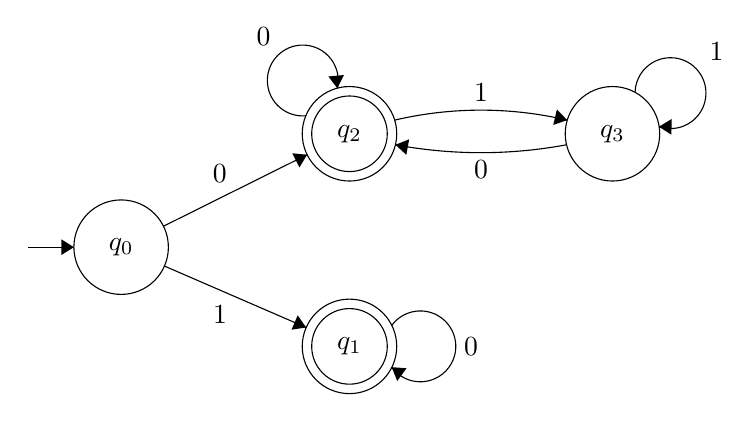
\begin{tikzpicture}[scale=0.2]
            \tikzstyle{every node}+=[inner sep=0pt]
            \draw [black] (15.4,-28.7) circle (3);
            \draw (15.4,-28.7) node {$q_0$};
            \draw [black] (29.9,-21.5) circle (3);
            \draw (29.9,-21.5) node {$q_2$};
            \draw [black] (29.9,-21.5) circle (2.4);
            \draw [black] (46.6,-21.5) circle (3);
            \draw (46.6,-21.5) node {$q_3$};
            \draw [black] (29.9,-35) circle (3);
            \draw (29.9,-35) node {$q_1$};
            \draw [black] (29.9,-35) circle (2.4);
            \draw [black] (18.09,-27.37) -- (27.21,-22.83);
            \fill [black] (27.21,-22.83) -- (26.27,-22.74) -- (26.72,-23.64);
            \draw (21.66,-24.6) node [above] {$0$};
            \draw [black] (32.77,-20.633) arc (103.21485:76.78515:23.971);
            \fill [black] (43.73,-20.63) -- (43.07,-19.96) -- (42.84,-20.94);
            \draw (38.25,-19.5) node [above] {$1$};
            \draw [black] (27.139,-20.356) arc (275.21649:-12.78351:2.25);
            \draw (24.44,-15.93) node [above] {$0$};
            \fill [black] (29.13,-18.61) -- (29.55,-17.77) -- (28.56,-17.86);
            \draw [black] (43.684,-22.198) arc (-79.43146:-100.56854:29.626);
            \fill [black] (32.82,-22.2) -- (33.51,-22.84) -- (33.69,-21.85);
            \draw (38.25,-23.2) node [below] {$0$};
            \draw [black] (48.037,-18.88) arc (178.99202:-109.00798:2.25);
            \draw (52.73,-16.27) node [right] {$1$};
            \fill [black] (49.55,-21.05) -- (50.34,-21.56) -- (50.36,-20.56);
            \draw [black] (18.15,-29.9) -- (27.15,-33.8);
            \fill [black] (27.15,-33.8) -- (26.61,-33.03) -- (26.22,-33.94);
            \draw (21.68,-32.36) node [below] {$1$};
            \draw [black] (32.58,-33.677) arc (144:-144:2.25);
            \draw (37.15,-35) node [right] {$0$};
            \fill [black] (32.58,-36.32) -- (32.93,-37.2) -- (33.52,-36.39);
            \draw [black] (9.5,-28.7) -- (12.4,-28.7);
            \fill [black] (12.4,-28.7) -- (11.6,-28.2) -- (11.6,-29.2);
            \end{tikzpicture}
            \end{center}
            
        \caption{A (a example of DFA)}
    \end{figure}
    In A, we see that\\
    $0110$ is accepts, since $q_0\to q_2$.\\
    $0101$ is rejected, since $q_0\to q_3$.
\end{example}
\begin{definition}[State transition]
    $\delta: Q\times \Sigma \to Q$ is the transition function.
    \begin{center}
        $\delta(q,a) = q'$ means that there is a edge labeled $a$ from $q$ to $q'$.
    \end{center}
\end{definition}

\begin{definition}[deterministic finite state automaton DFA]
    Formally, a DFA is a 5-tuple
    \[M = (Q,\Sigma,\delta, q_0,F)\]
    where $Q,\Sigma,\delta, q_0,F$ are defined in Example \ref{exa:DFA}.
\end{definition}
\begin{definition}[Extended transition function]
    $\delta^*: Q\times \Sigma^*\to Q$ is a extended transition function
    {\normalfont\scshape Base cases}: $\delta^*(q,\lambda) = q$\\
    {\normalfont\scshape Constructor cases}: for all $a\in \Sigma, x\in \Sigma^*$, we have $\delta^*(q,xa) = \delta(\delta^*(q,x),a)$.\\ 
    Alternatively, $\delta^*(q,ax) = \delta^*(\delta(q,a),x)$\\
    If $\delta^*(q,x)= q'$, we say that $x$ takes the automaton $M$ from $q$ to $q'$.
\end{definition}
\begin{definition}[the language accepted by $M$]
    $\mathcal{L}(M) = \{x\in \Sigma^*| M \mbox{ accepts } x\}$\\
    Also, $\mathcal{L}(M) = \{x\in \Sigma^*| \delta^*(q_0,x)\in F \}$
\end{definition}
\begin{proof}[Proof of Example \ref{exa:DFA}]Denote
    $\mathcal{L}(A) = \{x\in \{0,1\}^*|\mbox{ $x$ begin with $1$ or $x$ begin and end with $0$} \}$\\
    We first associate a set of strings (why is not language?) $L_i$ with each state $q_i$.
    \[L_i = \{x\in \Sigma^*|\delta^*(q_0,x)= q_i\}\]
    Prove by structural induction or induction on the length of $x$.\\
    We see that
    \begin{align*}
        L_0 &= \{\lambda\}\\
        L_1 &= \{x|\mbox{ $x$ start with 1}\} = \mathcal{L}(1(0+1)^*)\\
        L_2 &= \{x\in\{0,1\}^*|\mbox{$x$ starts and end with 0}\} = \mathcal{L}(0(0+1)^*0+0)\\
        L_3 &= \{x\in\{0,1\}^*|\mbox{$x$ starts with 0 and end with 1}\}
    \end{align*}
    Then we can prove $L' = L_1\cup L_2$.
\end{proof}

\section{Nondeterministic Finite Automaton NFA}

\begin{definition}[NFA]
    \[M = (Q,\Sigma, \delta, q_0,F)\]
    The only difference to DFA is that\[\delta: Q\times \Sigma\to \mathcal{P}(Q)\]
    $M$ acceptes the string $X$, if there is a path from $q_0$ to accept state labeld by $X$.
\end{definition}
\begin{definition}[Extended transition function]
    Denote the extended transition function $\delta^*:Q\times \Sigma\to \mathcal{P}(Q)$ as
    \begin{align*}
        &\mbox{\normalfont\scshape Base Case:} &\delta^*(q,\lambda) &= \{q\}\\
        &\mbox{\normalfont\scshape Constructor Case:} &\delta^*(q,xa) &= \bigcup\{\delta(q',a)|q'\in \delta^*(q,x)\}
    \end{align*}
\end{definition}\begin{definition}[The language that $M$ accepts]
    \[\mathcal{L}(M) = \{x\in \Sigma^*|\delta^*(q_0,x)\cap F\neq \emptyset\}\]
\end{definition}
\newpage
\section{DFA NFA and variant of NFA}
\begin{recall}
    A finite automaton is a 5-tuple
$M = (Q,\Sigma, \delta, q_0, F)$
\begin{align*}
    \mbox{DFA }&\delta:Q\times \Sigma \to Q\\
    \mbox{NFA }&\delta:Q\times \Sigma \to \mathcal{P}(Q)
\end{align*}
The language $L(M)$ accept by $M$ is
\begin{align*}
    \mbox{DFA: }&\{x\in \Sigma^*|\delta^*(q_0,x)\in F\}\\
    \mbox{NFA: }&\{x\in \Sigma^*|\delta^*(q_0,x)\cap F \neq \varnothing\}
\end{align*}
\end{recall}

\begin{theorem}
    For every NFA $M=(Q,\Sigma, \delta, q_0, F)$ there is a DFA $M' = (Q',\Sigma', \delta', q_0', F')$\\ 
    such that $L(M')=L(M)$
    \begin{proof}
        \begin{formal}\ul
            Let $M=(Q,\Sigma, \delta, q_0, F)$ be an arbitrary NFA.\ul
            {\itshape Idea: keep track of the states that $M$ can be as it reads the input string.}\ul
            Let $M' = (Q',\Sigma', \gamma', q_0', F')$ be defined as follows:\ul
                \n $Q' = \mathcal{P}(Q)$\ul
                $q_0' = \{q_0\}$\ul
                $F'= \{s\in P(Q) = Q'|S\cap F \}$\ul
                $\Sigma' = \Sigma$ and $\delta = \delta'$\ul
                Denote $\gamma: Q'\times \Sigma \to Q'$ such that\ul
                $\gamma(s,a) = \bigcup\{\delta(q,a)|q\in s\}$ for all $s\in Q'$ and $a\in \Sigma$.\ul
            
            \p  This is called subset construction.\ul\ul
            Claim $L(M) = L(M')$\ul
            For all $w\in \Sigma^*$, let $P(w) := ``\gamma^*(\{q_0\},w) = \delta^*(q_0,w)"$\ul
            Now show that $\forall w\in \Sigma^*. P(w)$ by structural induction\ul
            {\scshape Base Case}: $w = \lambda$\ul\n 
                By definition of extended transition function, we know\ul
                \n $\gamma^*(\{q_0\}, \lambda) = \{q_0\} = \delta^*(q_0,\lambda)$\ul\p 
            \p {\scshape Constructor Case}: $w = xa$, where $x\in \Sigma^*$ and $a\in \Sigma$\ul\n 
                Assume $P(x)$, i.e., $\gamma^*(\{q_0\}, x) = \delta^*(q_0,x)$\ul
                $\gamma^*(\{q_0\},w) = \gamma(\gamma^*(\{q_0\},x),a)$ by definition \ul
                \n\n\n\quad$ =\bigcup\{\delta(q,a)|q\in \gamma^*(\{q_0\},x)\}$ by construction\ul
                \quad$ =\bigcup\{\delta(q,a)|q\in \delta^*(q_0,x)\}$ by substitution\ul
                \quad$ =\delta^*(q_0,w)$ by definition\ul\p\p
                \p So $P(w)$ is true.\ul
            \p  By induction, $\forall w\in \Sigma^*. P(w)$
        \end{formal}
        Therefore, $w\in \mathcal{L}(M') \iff \gamma^*(\{q_0\}, w)\in F'\iff \gamma^*(\{q_0\}, w)\cap F\neq \varnothing\iff w\in \mathcal{L}(M)$
    \end{proof}
\end{theorem}
\section{Variants of NFAs}
\subsection{NFA with multiple initial states}
\[M= (Q,\Sigma, \delta, I, F)\]
where $I\subseteq Q$
\[L(M) = \{x\in \Sigma^*|\exists q\in I.(\delta^*(q,x)\cap F\neq \varnothing)\}\]
i.e., $M$ acceptes $x$ if and only if there is a path from some initial state to a final state labelled by $x$.
\begin{corollary}
    if $L$ is accepted by an NFA with multiple start start $s$, then it is accepted by an NFA.\\
    we can construct a normal NFA $M'(Q\cup \{q_0\},\sigma, \delta',q_0, F' )$, where $q_0\not \in Q$, such that
    \[\delta'(q_0,a) = \bigcup\{\delta(q,a)|q\in I\} \mbox{ for all $a\in \Sigma$}\]
    \[\delta'(q,a) = \delta(q,a)\mbox{ for all $q\in Q, a\in \Sigma$}\]
    \begin{equation*}
        F' = \left\{\begin{aligned}
            &F &\mbox{\normalfont if }\ I\cap F = \varnothing\\
            &F\cup\{q_0\} &\mbox{\normalfont if }\ I\cap F\neq \varnothing
        \end{aligned}
            \right.
    \end{equation*}
    \begin{proof}
        omit
    \end{proof}
\end{corollary}
\subsection{NFA with $\lambda$-transitions}
let $M= (Q,\Sigma, \delta, q_0, F)$ where \[\delta: Q\times (\Sigma\cup \{\lambda\}) \to \mathcal{P}(Q)\]
Denote $L(M)$ as
\[L(M) = \{x\in \Sigma^*|\delta^*(q_0,x)\cap F \neq \varnothing\}\]
$M$ accepts $x$ if and only if there is a path from $q_0$ to a final state such that\\ 
$x$ = concateration of the labels of the edges on that path.
\begin{corollary}
    if $L$ is accepted by an NFA with $\lambda$-transition, then it is accepted by an NFA.\\
    Denote $E(q) = \delta^*(q,\lambda) = \{q'\in Q|\mbox{ there is a path from $q$ to $q'$ labeled by $\lambda$}\}$\\
    Then we can construct a NFA with multiple innitial states $M'=(Q,\Sigma, \delta', E(q_0), F)$, where for all $q\in Q, a\in \Sigma$, 
    \[\delta'(q,a) = \bigcup\{E(q')|q'\in \delta(q,a)\}\]
    \begin{proof}
        omit
    \end{proof}
\end{corollary}
\section{Closure Results}
\begin{theorem}
    Suppose $L_1,L_2\subseteq \Sigma^*$ are accepted by finite automaton, then so are\\
        % \begin{tabularx}{\textwidth}{c c}
        %     \begin{align}
        %         \Sigma^*-L_1=\bar L_1

        %     \end{align}
        % \end{tabularx}
\end{theorem}
\end{document}